\documentclass[a4paper,oneside,10pt]{article}

\usepackage[dvipdfmx]{graphicx}
\usepackage{hyperref}
\hypersetup{final=true}
\setlength{\parskip}{1ex plus 0.5ex}
\newcommand{\submenu}{\begin{math}\rightarrow\end{math}}
\newcommand{\secref}[1]{(section \ref{sec:#1})}

\title{Using Pixylator (1.0 alpha)}
\author{K. Sehara}
\date{\vspace{-5ex}}

% 2017.5.15 First draft


\begin{document}

\maketitle

\hrule

\tableofcontents

\vspace{3ex}

\hrule

\newpage

\section{What is Pixylator?}
In short terms, Pixylator is a hue-based object categorization system that is implemented as an ImageJ plugin. The name ``Pixylator" derives from the Pixy camera (\url{http://charmedlabs.com/default/pixy-cmucam5/}), which reports the positions of color-coded objects at a rate of 60 samples per second (SPS). 
The idea and algorithm used in Pixylator plugin originate from those of Pixy camera.


The basic procedures are as follows:
\begin{enumerate}
\item Take movies using your favorite camera.
\item Open the movie in ImageJ (possibly convert it beforehand).
\item Run Pixylator on the movie.
\end{enumerate}



\section{Installation}
Once you downloaded the Pixylator file and extract it (in case it is a zip file), it should be a directory containing lots of files. 

\begin{enumerate}
\item Place the directory inside ``plugins" directory of ImageJ (it should be in the same directory as in the ImageJ app itself).
\item Restart ImageJ.
\item Open any color image file on ImageJ.
\item Find the submenu ``Pixylator" in the ``Plugins" menu (the items should be in an alphabetical order), and select ``Pixylator alpha" from it.
\item If you see the main window of the plugin, the installation is successful.
\end{enumerate}

In cases either 1) you cannot recognize the ``Pixylator" submenu in the ``Plugins" menu, or 2) you encounter (through the process) a log output complaining about something, then it is likely the plugin is compiled in a different version of ImageJ. Then:

\begin{enumerate}
\item Select menu ``Plugins" \submenu ``Compile and Run...".
\item Find and select ``Pixylator\_alpha.java" in the ``Pixylator" directory, which you have just moved in the ``plugins" directory.
\item See if the main window of the plugin pops up.
\end{enumerate}

Otherwise, please ask a person nearby that seems to know ImageJ plugins.



\section{Basics}
After opening your movie, open ``Pixylator" plugin. There, you can configure the tracking.

\subsection{Concepts and limitations}

\subsubsection{Hue-based object tracking}
Pixylator (just like Pixy) detects pixels that have the specified range of {\bf hues} (for the description of hue, refer to Wikipedia: \url{https://en.wikipedia.org/wiki/Hue}). It is believed to be less sensitive to the change in lightings than the brightness or the color itself.

Pixylator works as follows for each of the frames in the movie:
\begin{enumerate}
\item Calculate the hue for each of the pixels.
\item Collect the pixels that are within the specified range.
\item Generate the output, and go on to the next frame.
\end{enumerate}

\subsubsection{One object per one hue range}
Note that there is an important difference between Pixy and Pixylator. Whereas the former separates individual objects with the same hue range after step 2, the latter reports the set of pixels as one single ``set". In other words, for Pixylator there should be at maximum one object within one hue range.

\subsubsection{Only two classes are available}
Also, there are only two entries for hue ranges for the moment. This is just the simplicity and the utility reasons. The available number of entries may increase in the future.


\subsection{Typical procedures}
Note that the plugin is still in the alpha phase, and it can be buggy. It is {\bf highly recommended to generate/save ``mask images" (at least for some of the files; see section \ref{sec:output})  and visually verify that the objects be correctly identified, and that object locations be as expected}.

\begin{enumerate}
\item Open the image/movie file on ImageJ.
\item Open Pixylator plugin.
\item {\it (Optional)} Load existing configuration, if any.
\item Configure frames to track.
\item Configure the ROI to track.
\item {\it (Optional)} Re-plot the histogram and re-configure hue ranges.
\item {\it (Optional)} Rename the object names as you like.
\item Configure the output to generate.
\item {\it (Optional)} Save the current configuration.
\item Run tracking.
\item Inspect/save the results.
\item If you have another image/movie to process, open it and go on.
\end{enumerate}

You can find how to do each step for the rest of this document.





\section{Overview of the plugin GUI}
Below is the main panel for the plugin.

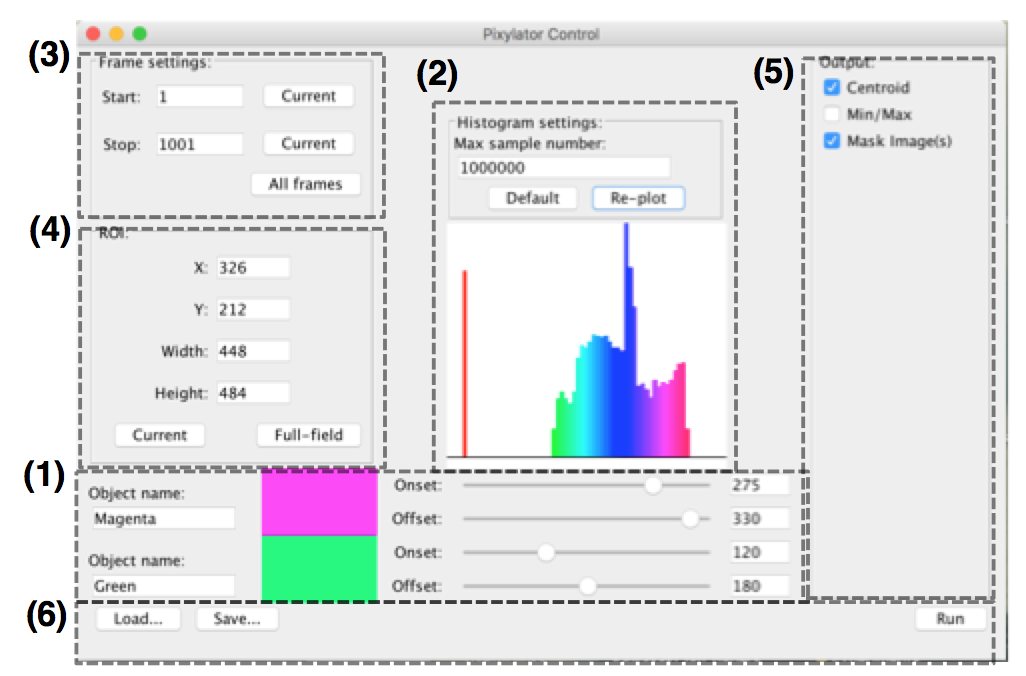
\includegraphics[width=10cm]{annotated.png}

Several components can be seen.
\begin{enumerate}
\item {\bf Mask control}: configuration for hue ranges to track.
\item {\bf Histogram}: a hue histogram of the movie file.
\item {\bf Frame settings}: configuration of which frames are to be used.
\item {\bf ROI settings}: configuration of the region to be used.
\item {\bf Output settings}: configuration of what output to generate.
\item {\bf Button panel}: a set of actions for the plugin.
\end{enumerate}

\subsection{Mask Control}
\label{sec:mask}
This is the core configuration of Pixylator. The Mask control interface is found near the bottom of the plugin. 

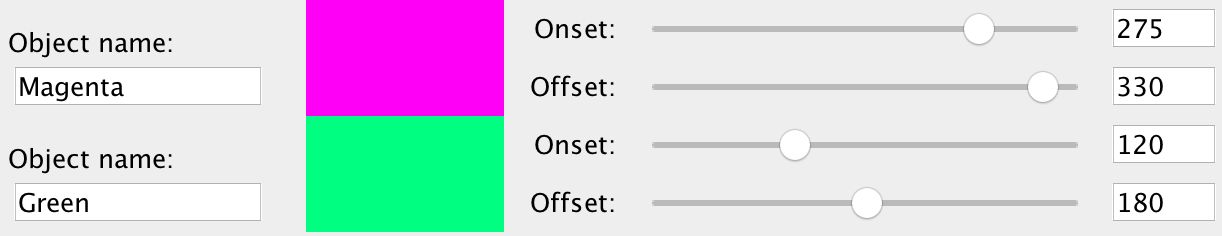
\includegraphics[width=10cm]{maskcontrol.png}

On the leftmost of the Mask Control interface, you can find text fields labeled as ``Object name: ". Here you can set the name of this object category to something more understandable to you.

Object names are used as the column names when the output \secref{output} is generated.

Next to the object names, you can see colored rectangles. This is the representative color for the hue range at the moment. As you change the hue range (see below), the color changes accordingly.

Note that the representative colors are used to draw masks when "mask images" are generated for the output \secref{output}.

The sliders and text fields that lie on the center of the window is for control of hue ranges. For each hue range, hue values larger than ``onset" and smaller than ``offset" are picked up. You can refer to the histogram \secref{histo} above for approximate color of the hue.



\subsection{Histogram}
\label{sec:histo}
Once you open the plugin, Pixylator tries to plot the hue histogram of the current image (i.e. the frontmost image that is open). It may take a while the process is done.

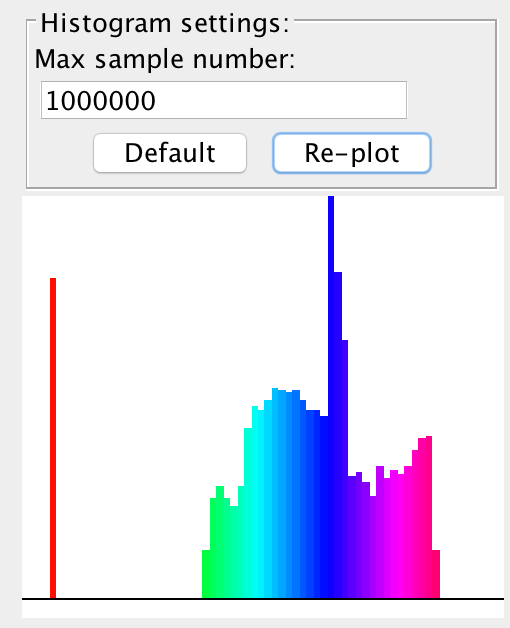
\includegraphics[width=6cm]{histogram.png}

By having a hue histogram, you can get a hint on what hue range to pick up as the object (note that the hue of the object often shows up as a mode in the histogram). The hue value is aligned with the slider for Mask  control \secref{mask}, so as to be easy to reflect the visual inspection results on the mask control.

The panel on the top of the histogram is the control for plotting. Because building a histogram is a heavy load for the plugin, it offers a way to perform sub-sampling of the image/movie file in a way the number of sampling not exceed ``Max sample number". The number goes back to the default value when you click on the ``Default" button.

You can change the range of pixels collected for generating histogram using Frame \secref{frame} or ROI \secref{roi} settings as well. In any case, make sure to click on ``Re-plot" button to update the histogram.


\subsection{Frame Settings}
\label{sec:frame}
On the top-left of the window, you can specify the controls for restricting frames used for tracking.

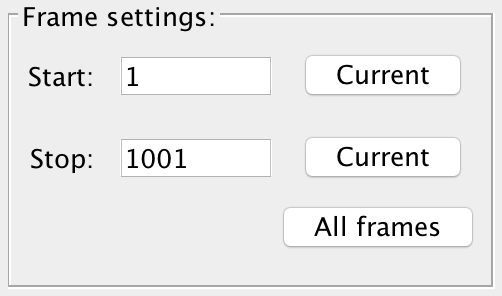
\includegraphics[width=6cm]{frame.png}

There are mainly two inputs: ``Start" and ``Stop". Here, ``Start" denotes for the first frame included for tracking, and ``Stop" for the last frame included for tracking. The frame number starts from 1. Thus, if you want to track 10 frames after the first 20 frames, then ``Start" is 21 and ``Stop" is 30.

Note that the selection of frames can affect histogram \secref{histo} generation as well. If you press ``Re-plot" button after changing Frame settings, the resulting histogram will only include pixels from the specified frames.

If you click on ``Current" button associated with either of the inputs, the current frame (the one that is visible on the image window) is selected as the corresponding input.

A click on ``All frames" let the plugin process all the images.


\subsection{ROI Settings}
\label{sec:roi}
On the middle-left of the window, you can find the ROI (for ``region of interest") settings to specify the region used for tracking.

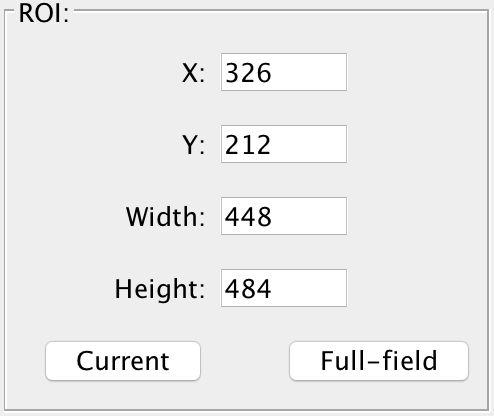
\includegraphics[width=6cm]{roi.png}

Restriction of ROI has both good and bad sides. Good things include 1) you can save time for computation, and 2) the data is less likely to get contaminated from unwanted object sources. On the other hand, arbitrary ROI selection may ``cut" the object as it moves in the movie. {\bf You need to be very careful that the ROI cover all of what you want}.


For the moment, the only way to specify the ROI is by using a rectangle: X and Y coordinates of the origin, the width, and the height.

The coordinate system follows the convention used in ImageJ. If you place the cursor somewhere on the image window, X and Y coordinates will be displayed on the space under the ImageJ tool bar (where lots of tool icons lie). Further, if you use the rectangular selection tool and perform a drag on the image window, you are likely to see the ``w" (stands for ``width") and ``h" (height) as well.

When you make a selection, and verified that the rectangle cover all the pixels of interest, you can click on ``Current" button of ROI settings. Then the coordinate data is transferred into Pixylator.

The button ``full-Field" sets the ROI back to the full field of view.


\subsection{Output Settings}
\label{sec:output}
On the right-hand side of the window is Output settings.

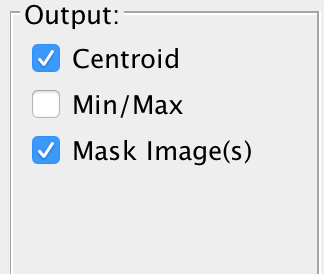
\includegraphics[width=5cm]{output.png}

\subsubsection{Parameter output}

Enabling ``Centroid" makes the plugin generate a table, and write centroid values for each of the object classes per each frame.

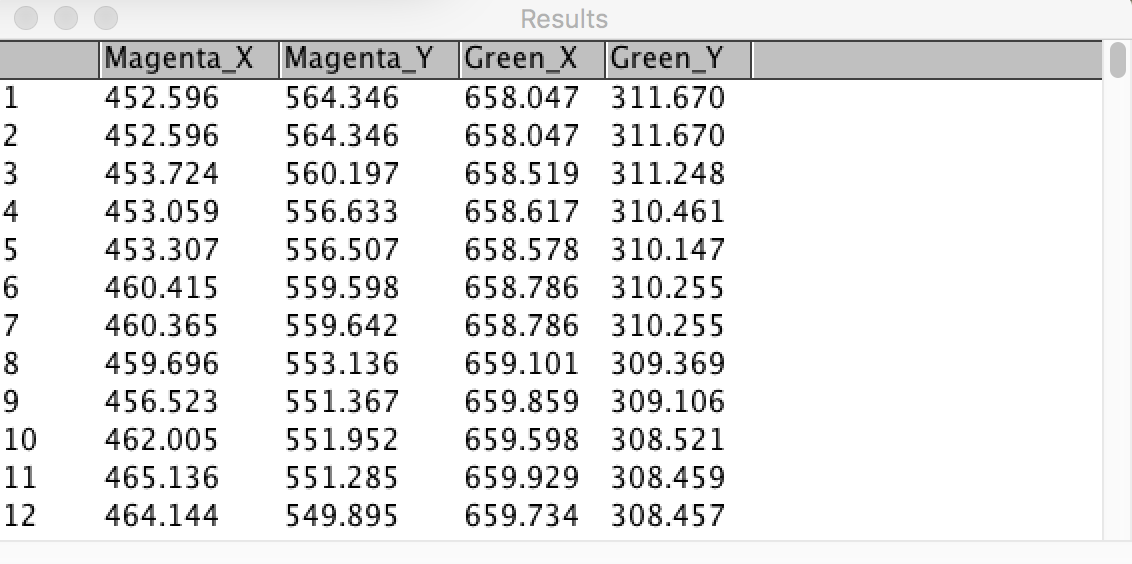
\includegraphics[width=8cm]{results.png}

Enabling ``Min/Max", on the other hand, writes the bounds of X- and Y-coordinates for each of the object classes. Both value types are written on a single Results window.


\subsubsection{Mask output}

When you enable ``Mask Image(s)", a whole new set of images are created. You can save the generated images in as many options as ImageJ provide.

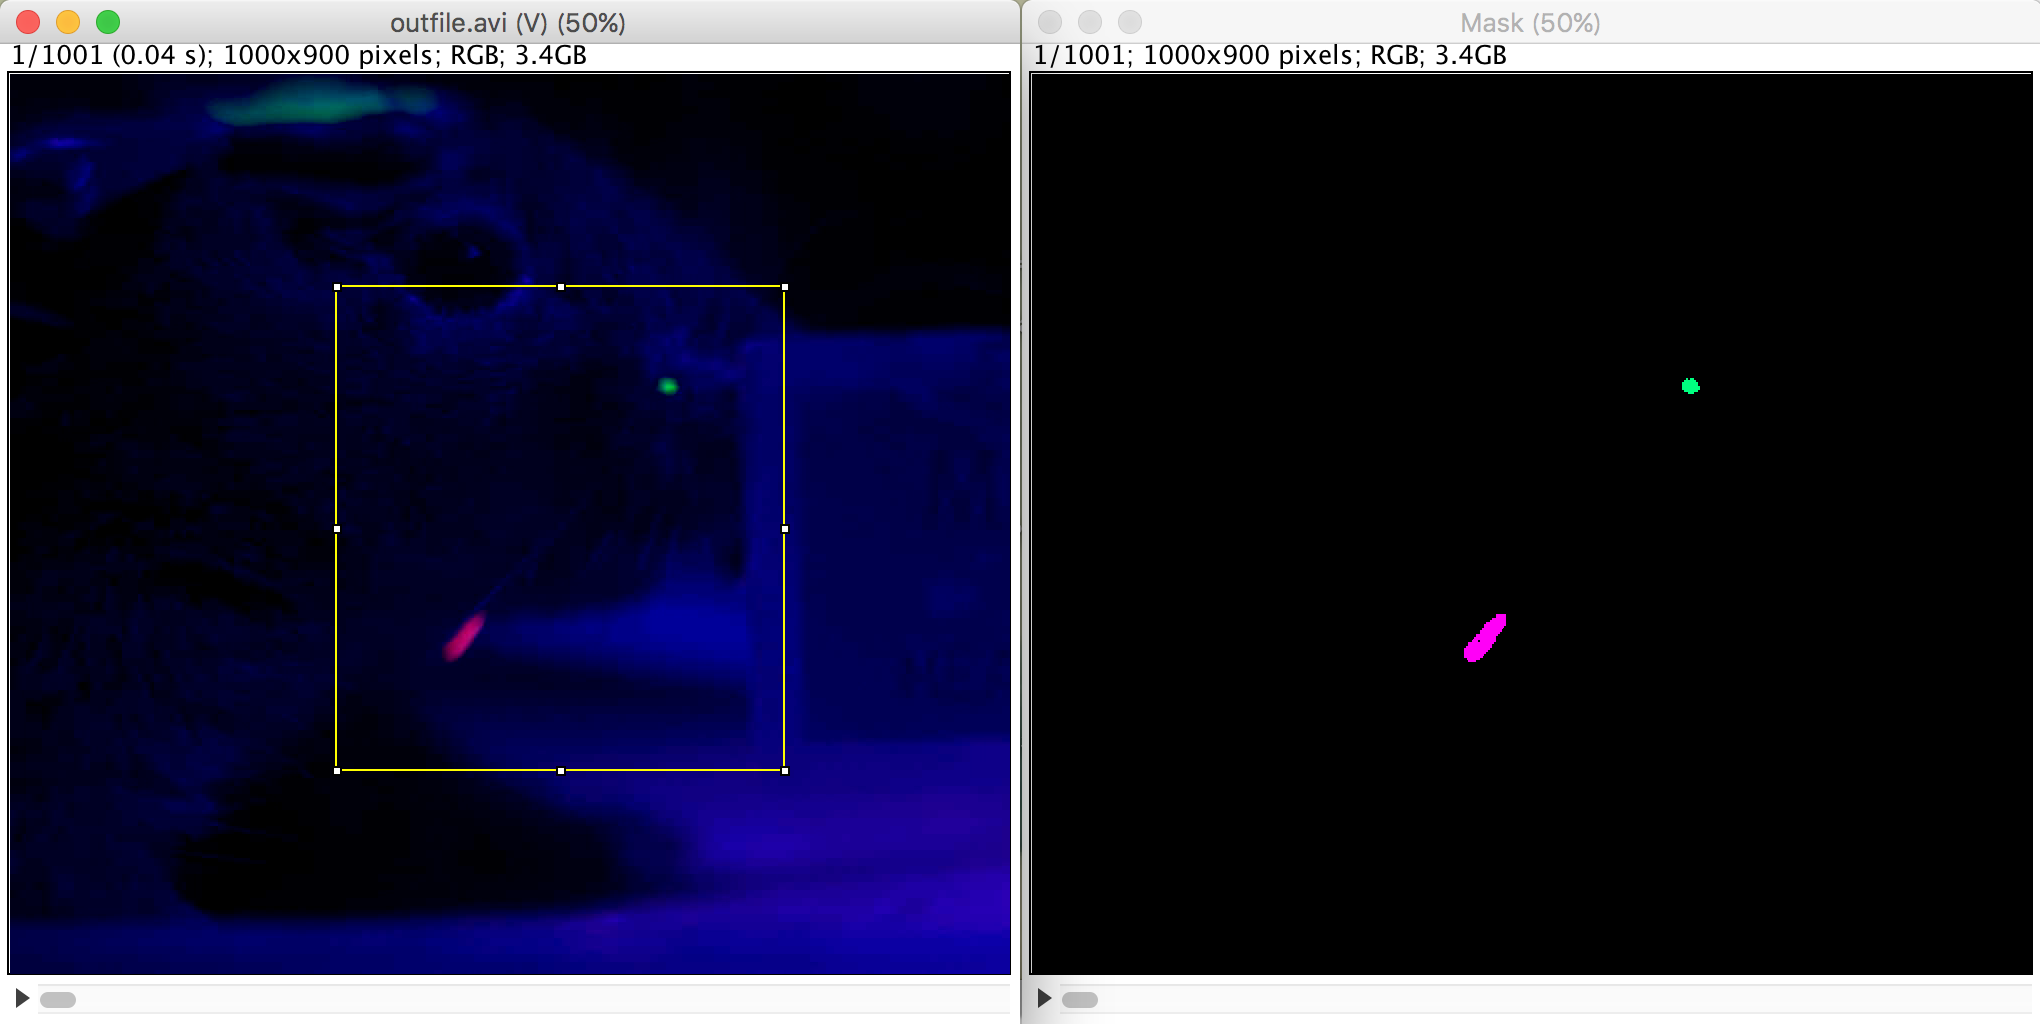
\includegraphics[width=10cm]{masks.png}

The highlighted area on the mask file represents the region (a set of pixels) whose hue value was within the specified range. The mask color is specific to the hue value range you used.

As you change the frames of the image set, you can see how Pixylator detected the objects in the specified frames.

Note that, even when you specified Pixylator to work within some small ROI (as in the case in the figure; ROI settings can be found at section \ref{sec:roi}), the mask image is created in the same size as the original movie. As such, the coordinate system is reconverted to the original one (in the parameter output as well).


\subsection{Actions}
On the panel at the bottom of the window, there are several actions that Pixylator can take.

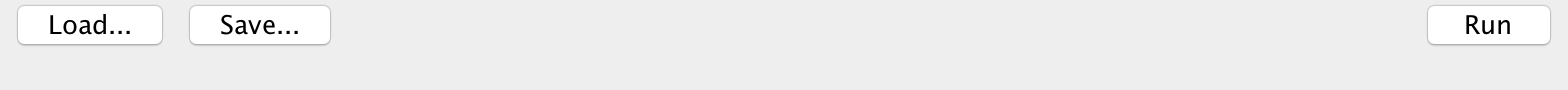
\includegraphics[width=14cm]{actions.png}

\begin{itemize}
\item {\bf ``Run" button}: runs the tracking using the current configurations.
\item {\bf ``Save..." button}: saves the current configurations to a file.
\item {\bf ``Load..." button}: loads the configurations that are saved into a file before.
\end{itemize}




\subsection{Troubleshooting}
Some of the problems that one may frequently encounter.

\subsubsection{ImageJ does not open the movie file}
Today, many movie files (even AVI files) are encoded in codecs such as h264, and ImageJ cannot open them.

You need to first decode them to obtain ``raw AVI files" for ImageJ to read them. Install and use tools such as {\bf ffmpeg}(\url{https://ffmpeg.org/}). Make sure to specify ``raw" AVI, and avoid any compression or encoding.

\subsubsection{I don't know what hue range I should choose}
This is the process that takes you most of the time. Below are some tips.

\paragraph{Start from simple}
Do not use 3600-frame movie first, but start from one representative single-frame (or up to 50 frames or so) image file. Alternatively, use Frame settings \secref{frame} to restrict the frames that you process.

\paragraph{Use standard colors}
In a single-frame image, specify the ROI that contains only the object (no background) \secref{roi}, and generate histogram \secref{histo}; by doing so several times, you will get an intuition about what hue value you are aiming for.

\paragraph{Verify what is obtained}
As you run several test runs using small-frame image samples, always generate ``Mask images" \secref{output}, and compare the results with your visual inspection:
\begin{itemize}
\item Is there any extra detection other than what you target? If so, try restricting the hue range \secref{mask} and/or restricting the ROI \secref{roi}.
\item Is there enough pixels detected for tracking on each frame? If so, you may need to widen the hue range.
\item Do the output centroid coordinates correspond nicely with the target object? There may be small ``pixel islands" that you may miss to detect, and that can cause errors on object tracking.
\end{itemize} 

\subsubsection{Hue histogram does not show up (or appear) properly}
\begin{itemize}
\item Check that the progress bar in the ImageJ toolbar is not working; if the number of pixels/frames is very large, drawing the histogram can take up to minutes. Change the ``Max sample numbers" and re-plot in those cases \secref{histo}.
\item Try clicking the ``Re-plot" button.
\item Try resizing the plugin window (although it is unlikely, repainting of the histogram is somehow stuck).
\item Check that the Frame/ROI settings are correct (sections \ref{sec:frame} and \ref{sec:roi}). If you re-use the plugin in the same ImageJ session, it is possible that the previous configurations contaminate the working of histogram.
\end{itemize}

\subsubsection{Things (histogram and/or tracking) are really slow}
It can be the problem of the computer/OS, but assume here that it is the problem of the plugin. Here are what one can take:
\begin{itemize}
\item Make the ROI smaller (but without cutting the objects to be tracked; see section \ref{sec:roi}).
\item Disable ``Mask Image(s)" output \secref{output}.
\item (For histograms only) reduce ``Max sample number" \secref{histo}.
\end{itemize}

\subsubsection{Too few results are generated as the output}
If you re-use the plugin in the same ImageJ session, it is possible that the previous configurations contaminate the working of tracking. Check that Frame/ROI settings are correct (see sections \ref{sec:frame} and \ref{sec:roi}).

\subsubsection{Cannot save the ``Mask images"}
If you deal with a movie that has many/large frames, it is likely that saving process hit the theoretical maximal size of a TIFF file (2 GB in most cases).

One of the best solutions is to split the image set into several stacks. You can do it by using ``Image" \submenu ``Stacks" \submenu ``Tools" \submenu ``Make Substack..." (Alternative way is to use ``Stk" button on the ImageJ toolbar, then select ``Make Substack..." from it). By checking ``Delete slices from original stack", you can successfully dissociate a set of frames from the rest. Then you can save the individual stacks as separate TIFF files.

In some cases, the split files can be merged back by compressing the frames (this is especially true for the case of Masked images). Use tools such as Libtiff. More specifically, a command called tiffcp (or TiffCP) takes care of both concatenating and compressing at once.

\begin{itemize}
\item {\bf for Windows} Install LibTiff.Net (\url{https://bitmiracle.com/libtiff/}), and run TiffCP on the command prompt (cmd.exe).
\item {\bf for Mac} Retrieve the source file and build it yourself (follow e.g. \url{http://mac-dev-env.patrickbougie.com/libtiff/}). Alternatively, you can install libtiff through package manager such as Homebrew (\url{https://brew.sh/}) 
\item {\bf for Linux} In many cases libtiff tools are already installed (check with ``which tiffcp"), but in case not, check for ``libtiff" in the package manager.
\end{itemize}

\subsubsection{ImageJ runs out of memory}
Change the volume of memory for ImageJ and restart the app; increase the available amount of memory at ``Edit" \submenu ``Options" \submenu ``Memory \& Threads...".

\end{document}